% MA211 - Lecture 16
\documentclass[pdftex, xcolor=pdftex, dvipsnames, handout]{beamer}

\usetheme{MA211}
\usepackage{thumbpdf}
\usepackage{wasysym}
%\usepackage{ucs}
\usepackage[utf8]{inputenc}
\usepackage{pgf,pgfarrows,pgfnodes,pgfautomata,pgfheaps,pgfshade}
\usepackage{verbatim}

\usepackage{eurosym}
\usepackage{euler}

\usepackage{calc}               % Simple computations with LaTeX variables
%\usepackage[hang]{caption2}     % Improved captions

\usepackage{graphicx}           % Standard graphics package

\usepackage{amsmath, amsthm, amssymb}


\newcommand{\fquad}{\mbox{\qquad}}
\newcommand{\bull}{$\bullet$ }

\newcommand {\I} {\mathcal I}
\newcommand {\calI} {\mathcal I}
\def\disint{\displaystyle\int}

\DeclareMathOperator{\D}{d}
\newcommand{\dydx}{\frac{\D y}{\D x}}

%\definecolor{gray}{rgb}{0.69, 0.69, 0.69} \newcommand{\gray}[1]{\textcolor{gray}{#1}}
\definecolor{dogreen}{rgb}{0.33, 0.42, 0.18} \newcommand{\dogreen}[1]{\textcolor{dogreen}{#1}}
\definecolor{maroon}{rgb}{.5,0.2,0.2}\newcommand{\maroon}[1]{\textcolor{maroon}{#1}}
\definecolor{greena}{rgb}{.1,0.581,0.1}\newcommand{\greena}[1]{\textcolor{greena}{#1}}

\definecolor{blue4}{rgb}{0,0,.545}
\newcommand{\Blue}[1]{\textcolor{blue}{#1}}
\newcommand{\Red}[1]{\textcolor{red}{#1}}
\definecolor{pink}{rgb}{1.,0.75,0.8}
\definecolor{darkred}{rgb}{0.5,0.0,0.0}
\definecolor{darkgreen}{rgb}{0,0.3,0.3}
\definecolor{purple}{rgb}{0,0.3,0.3}
\definecolor{darkblue}{rgb}{0.0, 0.0, .5}
\definecolor{dpurple}{rgb}{.3,.0,.3}
\newcommand{\Green}[1]{\textcolor{darkgreen}{#1}}
\newcommand{\DRed}[1]{\textcolor{darkred}{#1}}
\newcommand{\DBlue}[1]{\textcolor{darkblue}{#1}}
\newcommand{\Purple}[1]{\textcolor{dpurple}{#1}}
\newcommand{\Emph}[1]{\textcolor{darkred}{\textbf{\it #1}}}
\newcommand{\remph}[1]{\textcolor{darkred}{\textbf{\emph{#1}}}}
\newcommand{\bemph}[1]{\textcolor{darkblue}{\textbf{\emph{#1}}}}
\newcommand{\gemph}[1]{\textcolor{darkgreen}{\textbf{\emph{#1}}}}
\newcommand{\Bf}[1]{\textcolor{darkblue}{\textbf{#1}}}
\newcommand{\Gf}[1]{\textcolor{darkgreen}{\textbf{#1}}}
\newcommand{\Rf}[1]{\textcolor{red}{\textbf{#1}}}
\newcommand{\Rmf}[1]{\textcolor{red}{\mathbf{#1}}}

\newcommand{\Conj}[1]{\overline{#1}}

\newcommand{\code}[1]{\textcolor{darkblue}{\texttt{\textbf{#1}}}}
\newcommand{\icode}[1]{{\blue\texttt{\textbf{\emph{#1}}}}}
\newcommand{\gcode}[1]{{\Green{\texttt{\textbf{\emph{#1}}}}}}
\newcommand{\out}[1]{\texttt{\emph{\textbf{\Green{#1}}}}}





\newenvironment{vminipage}%
{\begin{Sbox}\begin{minipage}\begin{small}\begin{verbatim}}%
{\end{verbatim}\end{small}\end{minipage}\end{Sbox}\fbox{\TheSbox}}

\newenvironment{nminipage}%
{\begin{Sbox}\begin{minipage}}%
{\end{minipage}\end{Sbox}\fbox{\TheSbox}}


\let\Arg\relax\DeclareMathOperator{\Arg}{\mathtt{Arg}}
\let\Arg\relax\DeclareMathOperator{\e}{\mathtt{e}}

\newcommand {\AND} {\wedge}
\newcommand {\OR} {\vee}
\newcommand {\NOT} {\neg}
\newcommand {\IMPLIES} {\rightarrow}
%\newcommand {\IFF} {\leftrightarrow}
\renewcommand {\iff} {\Leftrightarrow}
\newcommand {\NAND} {\uparrow}
\newcommand {\NOR} {\downarrow}
\newcommand {\XOR} {\otimes}

\newenvironment{citemize}% Colour items
{\begin{description}}%
{\end{description}}

\newcommand {\maroonitem}{\item[\maroon{$\bullet$}]}

\newcommand {\gitem} {\item {\includegraphics[width=.4cm,angle=-10]{img/green-bullet-on-white.ps}}}
\newcommand {\ritem} {\item {\includegraphics[width=.4cm,angle=-10]{img/red-bullet-on-white.ps}}}
\newcommand {\yitem} {\item {\includegraphics[width=.4cm,angle=-10]{img/yellow-bullet-on-white.ps}}}
\newcommand {\bitem} {\item {\includegraphics[width=.4cm,angle=-10]{img/blue-bullet-on-white.ps}}}

\newcommand {\greenitem} {\item {\includegraphics[width=.4cm,angle=-10]{img/green-bullet-on-white.ps}}}
\newcommand {\reditem} {\item {\includegraphics[width=.4cm,angle=-10]{img/red-bullet-on-white.ps}}}
\newcommand {\yellowitem} {\item {\includegraphics[width=.4cm,angle=-10]{img/yellow-bullet-on-white.ps}}}
\newcommand {\blueitem} {\item {\includegraphics[width=.4cm,angle=-10]{img/blue-bullet-on-white.ps}}}

\newcommand {\eq}[1]%
  {$\DBlue{#1}$}
\newcommand {\eqd}[1]%
  {$\displaystyle\DBlue{#1}$}
%\newcommand{\eq}[1]{\boldmath \DBlue{$#1$}}


\newcommand {\csf}{\centerslidesfalse}
\newcommand {\cst}{\centerslidestrue}

\newcommand {\vecii}[2] {   \big(\begin{smallmatrix} #1 \\ #2 \end{smallmatrix}\big)}
\newcommand{\atwo}[2]{\left(\!\!\begin{array}{c} #1 \\ #2 \end{array}\!\!\right)}


\newcommand{\C}{\mathbb{C}}
\newcommand{\Q}{\mathbb{Q}}
\newcommand{\R}{\mathbb{R}}
\newcommand{\N}{\mathbb{N}}
\newcommand{\Z}{\protect\mathbb{Z}}  % protect for index.
\newcommand {\Rs}{ \mathbb{R}}
\newcommand {\Cs}{ \mathbb{C}}
\newcommand {\Rnn}{ \mathbb{R}^{n \times n}}
\newcommand {\Rn}{ \mathbb{R}^{n}}


\newcommand{\mblock}{%
\setbeamercolor*{block title}{bg=maroon,fg=white}
\setbeamercolor*{block body}{bg=white,fg=maroon}
}%

\newcommand{\bblock}{%
\setbeamercolor*{block title}{bg=Steel,fg=white}
\setbeamercolor*{block body}{bg=Mylightgray,fg=Steel}
}%

\newcommand{\gblock}{%
\setbeamercolor*{block title}{bg=Green,fg=white}
\setbeamercolor*{block body}{bg=Mylightgray,fg=darkgreen}
}%


\newcommand{\rblock}{%
\setbeamercolor*{block title}{bg=Red,fg=white}
\setbeamercolor*{block body}{bg=white,fg=Black}
}%


\newcommand{\TakeNotes}{
\includegraphics[width=2cm]{TakeNote}}

\def\eps{\varepsilon}
\newcommand {\del}[2]{ {\frac{\partial #1}{\partial #2}}}
\newcommand {\x}[1]{x^{[#1]}}
\newcommand {\delx}{ {\frac{\partial}{\partial x}}}
\newcommand {\delt}{ {\frac{\partial}{\partial t}}}
\newcommand {\dely}{ {\frac{\partial}{\partial y}}}
\newcommand {\ith}{{(i)}}
\renewcommand {\vec}[1]{ {\boldsymbol{#1}}}
\newcommand {\Oh} {\mathcal O}
\newcommand {\Err} {\mathcal E}


\DeclareMathOperator{\E}{e}

\newcommand {\Rsym}{{ \mathbb{R}^{n \times n}_\mathrm{sym}}}

\newcommand {\st} {\mathrm{st}}
\newcommand {\nd} {\mathrm{nd}}


\parskip .25cm


\theoremstyle{definition}
\newtheorem{exercise}{Exercise}[section]
\newtheorem{method}{Method}[section]

\newcommand{\Header}[1]{\begin{center}{\Large \Bf{#1}}\end{center}}

\subtitle{MA211}
\title{Lecture 16: Series Solutions. Integration}

\author{Dr Niall Madden}

\date{\Large Mon $3^\mathrm{rd}$ Nov 2008}


\begin{document}

\setcounter{framenumber}{-1}
\frame{

\begin{block}{}
\begin{center}
{\large \insertsubtitle}

\vspace{.1cm}

\begin{large}
\textbf{\inserttitle}
\end{large}

\vspace{.15cm}

% {\footnotesize \insertauthor}

\vspace{.3cm}

{ {\insertdate}}
\end{center}
\end{block}


\vspace{-0.25cm}
\begin{center}
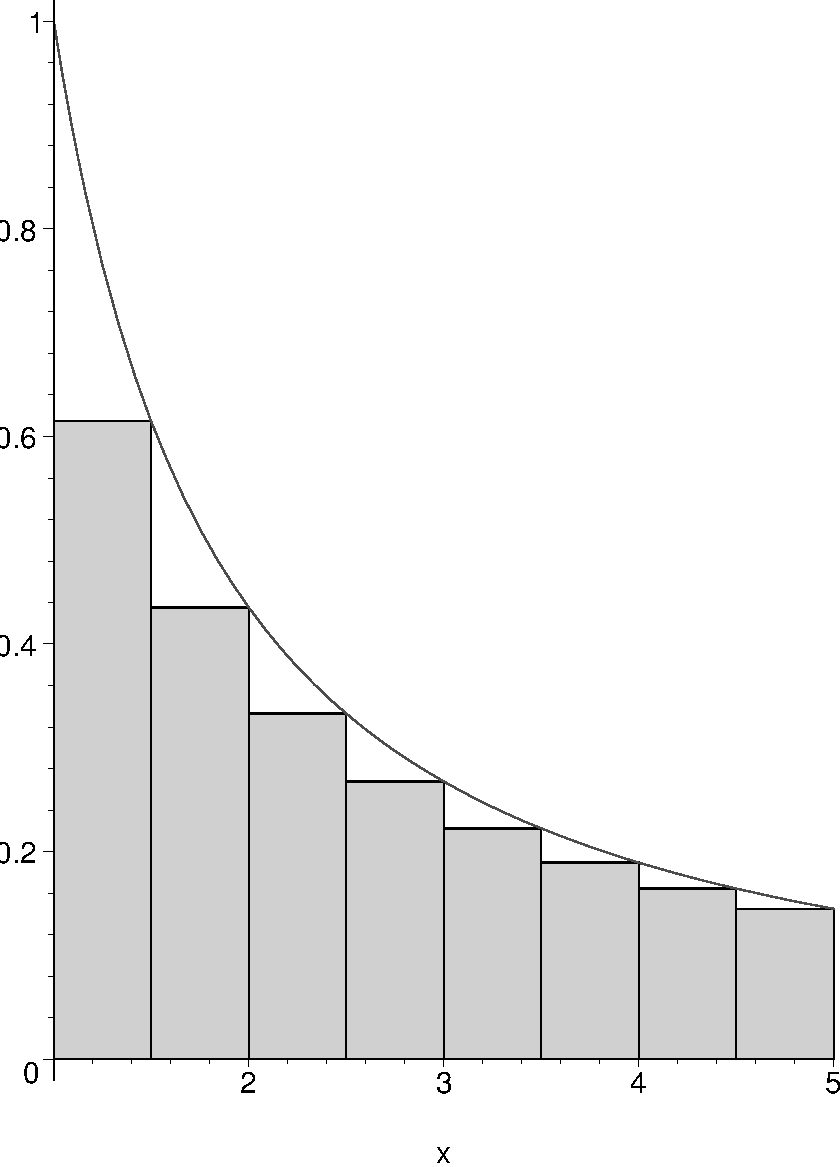
\includegraphics[width=4cm,height=4cm]{images/Box8}
\end{center}
}




\frame{
  \frametitle{Today...}

\begin{columns}[c]
\column{0.5\textwidth}
 \tableofcontents

\column{0.5\textwidth}

For more on \Emph{Series Solutions}, see Section 17.4 of Stewart
\Emph{Calculus: early transcendentals}.

~


For further examples on \Emph{Integration}, have a look at Chapter 5, but
especially Sections 5.5, 
\end{columns}
}




\section{Power Series}

\frame{

  Toward the end of last Wednesday's class, we started a section on
  \Bf{Series Solutions}.

This is a technique that allows use to write down approximate
solutions to problems with  \Emph{nonconstant   coefficients}.

For example
\[ y'' - xy' + y = 0.\]


}


\frame{

\begin{alertblock}{Power Series}
The key idea is that we suppose that we can write \eq{y} as 
\[
y = c_0 + c_1 x + c_2x^2 + c_3x^3 + \cdots = \sum_{n=0}^\infty c_n
x^n.\]
\end{alertblock}

The general solution will always have arbitrary constants, so we let
these be \eq{c_0} and \eq{c_1}. 

Then we substitute the power series is into the differential equation, and get
equations for \eq{c_2}, \eq{c_3}, \eq{c_4}, ...

The more terms we take, the more accurate the solution is.
 

}



\frame{
\begin{example}
Use a power series to solve the DE
\[y'' - x y = 0.\]
\end{example}


\vspace{4cm}

}


\subsection{Initial Value problems}
\frame{
Power series methods are particularly useful for getting solutions to
\emph{initial value problems} where we are given, not only the
differential equation, but also the value of \eq{y} and \eq{y'} at
some initial point.

These allow us to solve for \eq{c_0} and \eq{c_1}.


}

\frame{
\begin{example}
Use a power series to solve the initial value problem
\[y'' - x y = 0, \qquad y(0)=0, y'(0)=1.\]
\end{example}


\vspace{4cm}

}

\frame{

\begin{center}
\only<5>{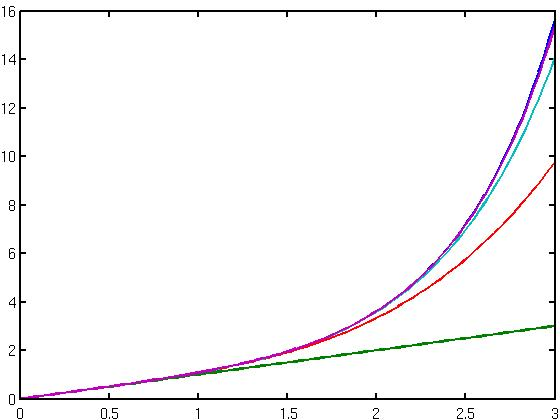
\includegraphics[height=7cm]{images/Series4}}
\only<1>{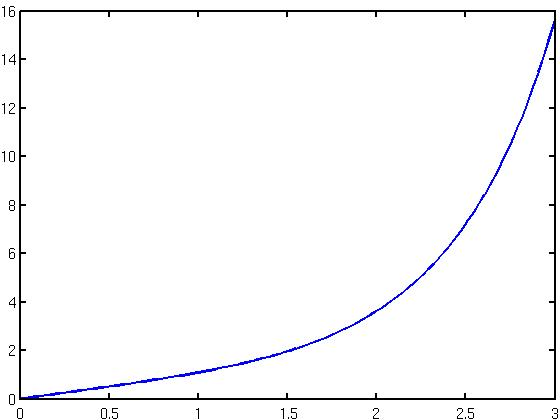
\includegraphics[height=7cm]{images/Series0}}
\only<2>{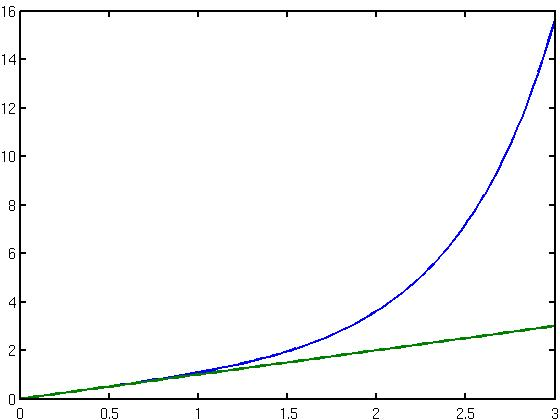
\includegraphics[height=7cm]{images/Series1}}
\only<3>{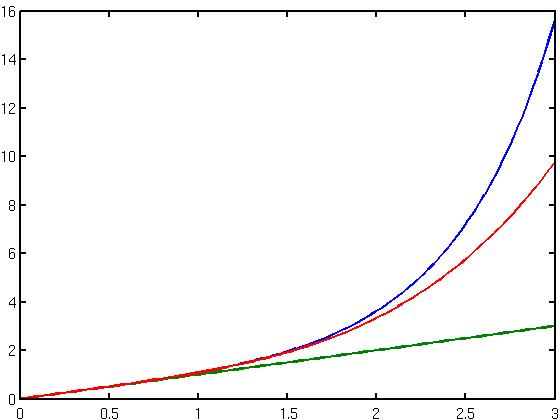
\includegraphics[height=7cm]{images/Series2}}
\only<4>{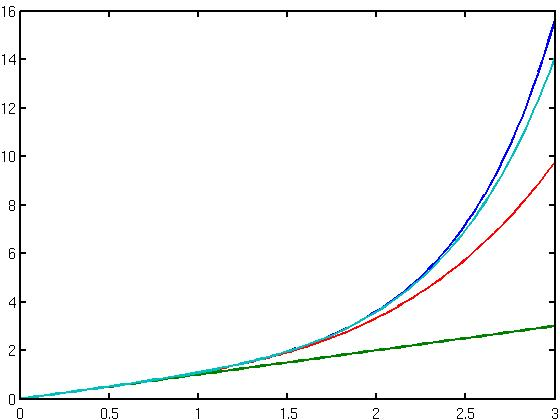
\includegraphics[height=7cm]{images/Series3}}
\end{center}

}
\frame{

\begin{exercise}[Q16.1]

For each of the following differential equations, find a recurrence
relation for the coefficients of  the power   series solution, and 
write out the solution up to the \eq{x^5} term.

\begin{enumerate}
\item $y'' + xy =0.$
\item $y'' + x^2 y =0.$

\item $y'' - 2xy' + y=0.$

\item $y'' - 2xy' + y=0, \quad y(0)=1, y'(0)=-1$

\item $y'' - xy' =0, \qquad y(0)=0, y'(0)=2$
\end{enumerate}



\end{exercise}
}



\section{Integration}
\frame{

We've now finished the section on solving  2nd order problem.

For the next few lectures we will study

\begin{alertblock}{New Section}
\begin{center}
\begin{Large}
\textbf{INTEGRATION}

\begin{columns}[c]
\column{0.3\textwidth}
{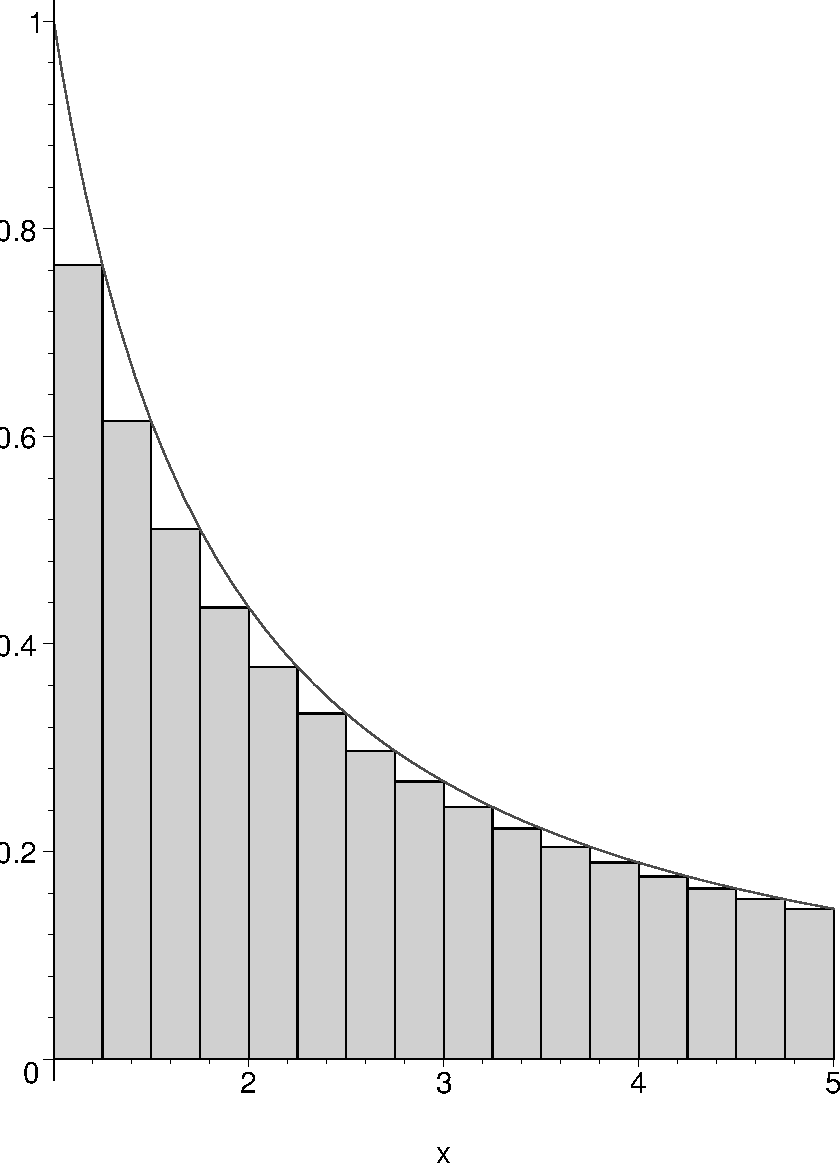
\includegraphics[width=5cm, height=3cm]{images/Box16}}
\column{0.3\textwidth}
\eqd{\approx \int_a^b f(x) dx}
\end{columns}
\end{Large}
\end{center}
\end{alertblock}

Later we'll return to the topic of solving 1st order problems.


}

\frame{

In this section of the course we return to the problem of:
\begin{block}{}
Given a function \eq{F}, find a function \eq{f} such that 
\[
f'(x) = F(x).
\]
We call \eq{f} an \Emph{anti-derivative} if \eq{F}.
(See Lecture 6)
\end{block}
More often we write this as an \Emph{Integral} problem:
\begin{block}{}
Given a function \eq{F}, find 
\[
f(x) = \int F(x) dx.
\]
\end{block}
}

\subsection{Preliminaries}
\frame{
\begin{block}{Sigma Notation}
We can write a sum \eqd{f_0, f_1, f_2, \dots, f_n}
as \eqd{\sum_{k=0}^n f_k.}
\end{block}

\begin{example}
\[1+2+3+4+\dots + 10 = \sum_{k=1}^{10} k.\]

\[1+3+5+7+\dots + 13 = \sum_{k=1}^7 (2k-1).\]
\end{example}
}

\section{Area Under a Curve}
\frame{
One can approximate the area from \eq{a} to \eq{b} bounded above by a
given function, below by the \eq{x}-axis by the area of boxes under
the curve:
\begin{center}
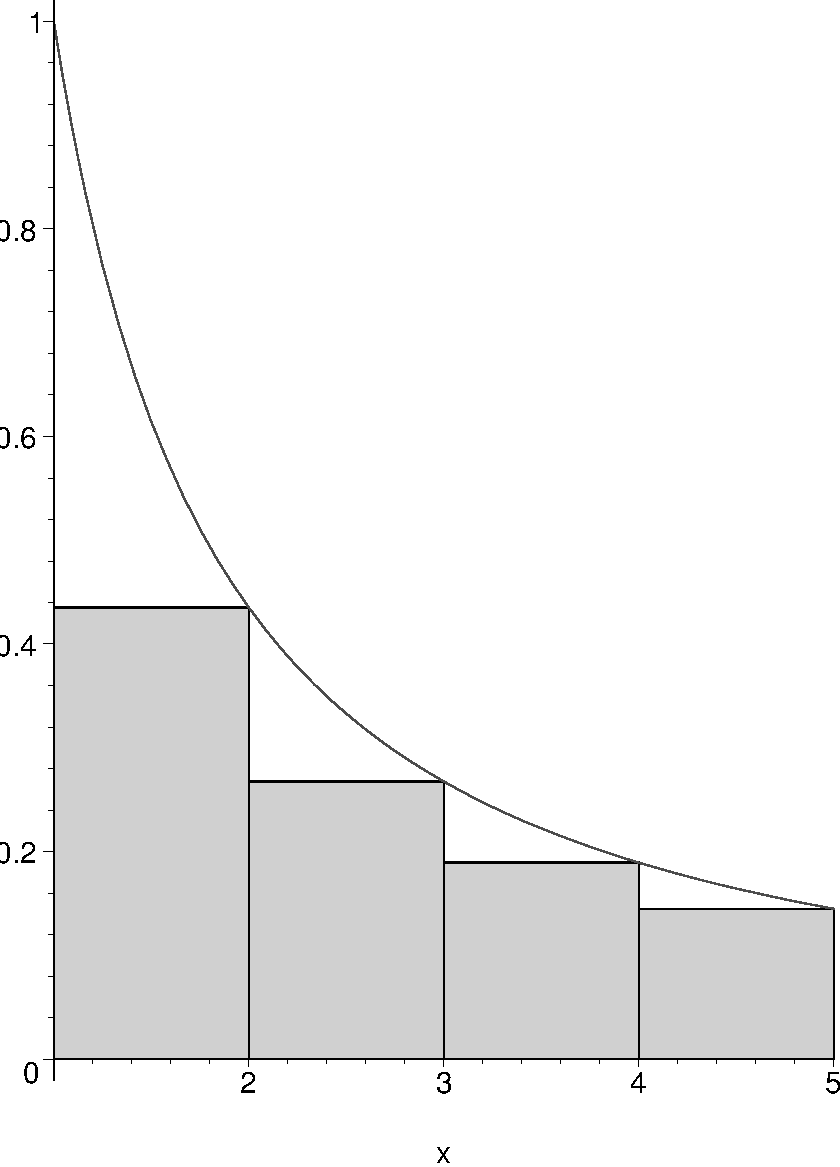
\includegraphics[width=8cm, height=5cm]{images/Box4}
\end{center}
\vspace{-0.5cm}
\[Area \approx A_1 + A_2 + A_3 + A_4 = S_4 = \sum_{k=1}^4 A_k.\]
}

\frame{
As we increase the number of boxes, the approximation improves...
\begin{center}
\only<5>{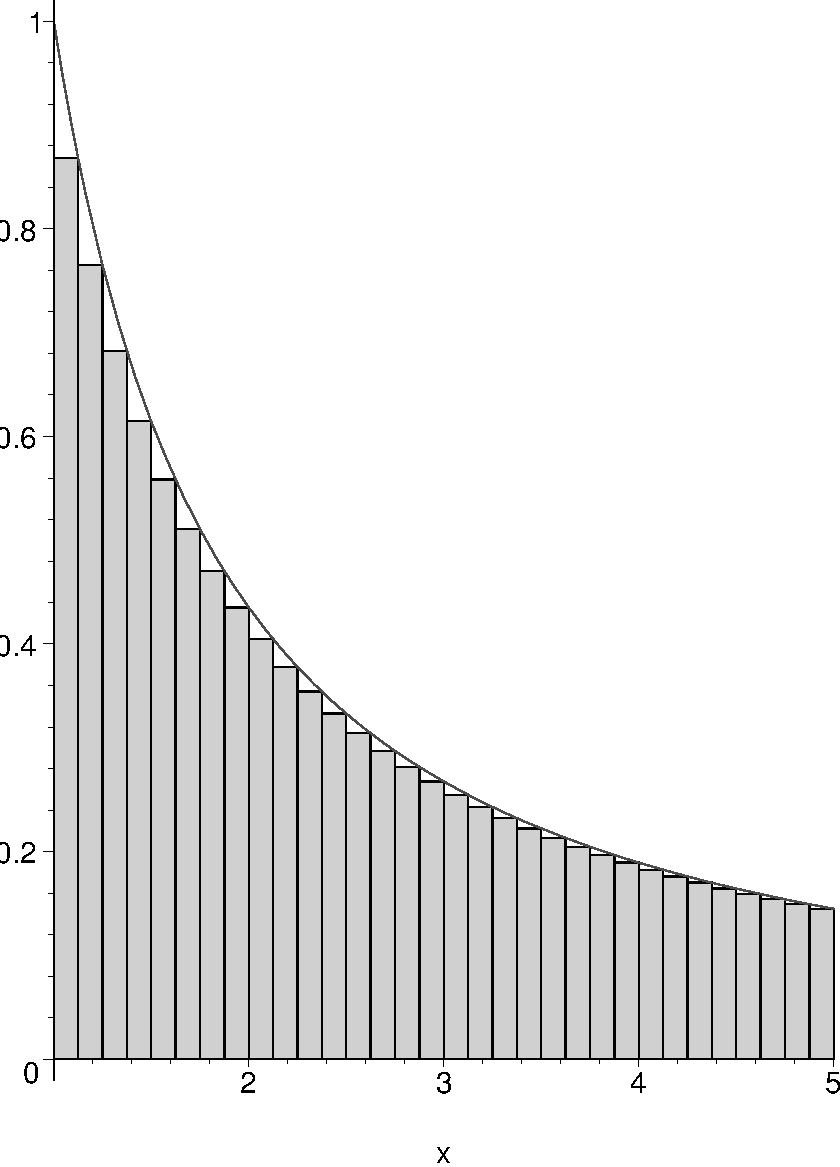
\includegraphics[width=8cm, height=6cm]{images/Box32}}
\only<1>{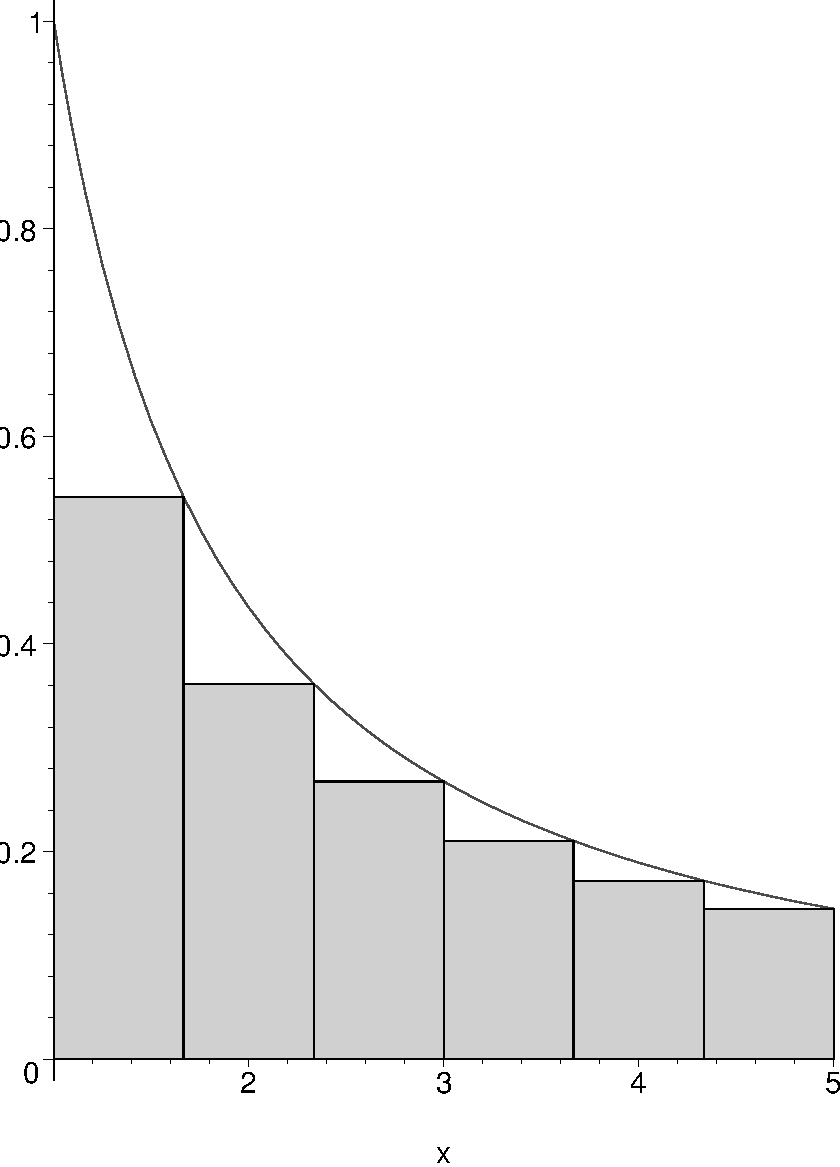
\includegraphics[width=8cm, height=6cm]{images/Box6}}
\only<2>{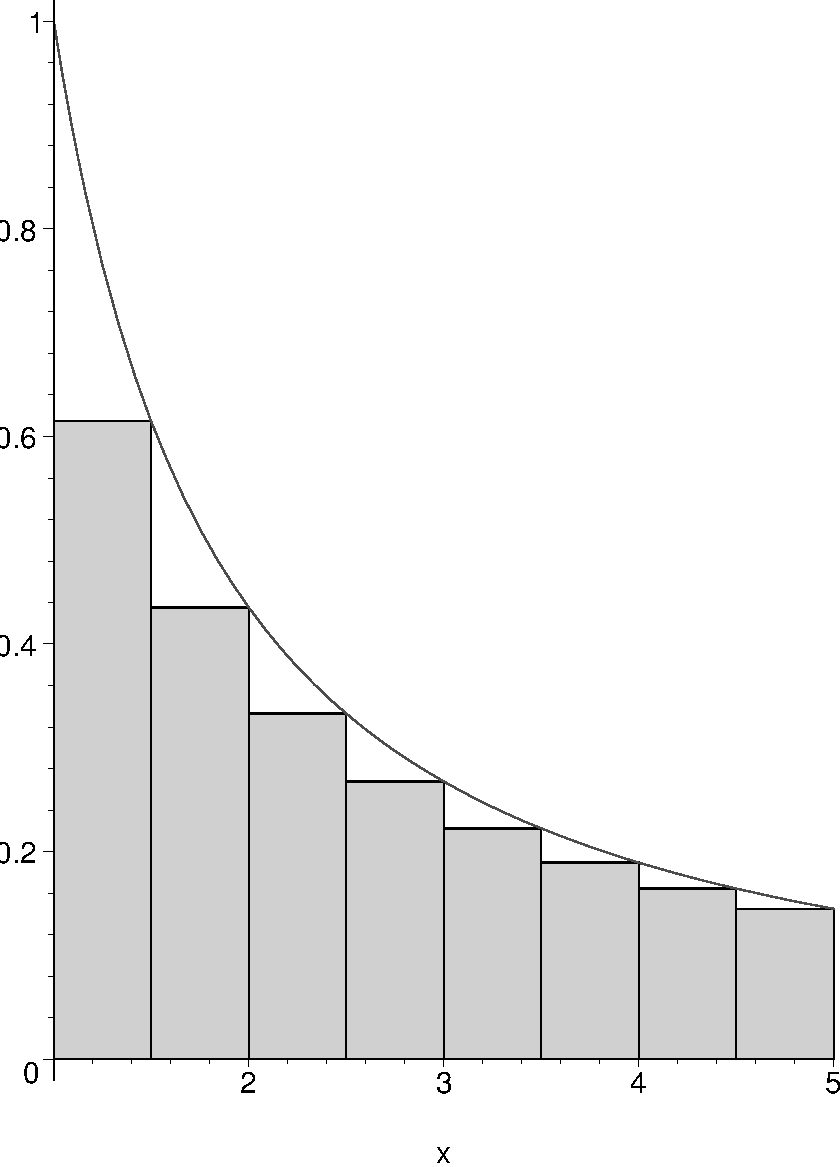
\includegraphics[width=8cm, height=6cm]{images/Box8}}
\only<3>{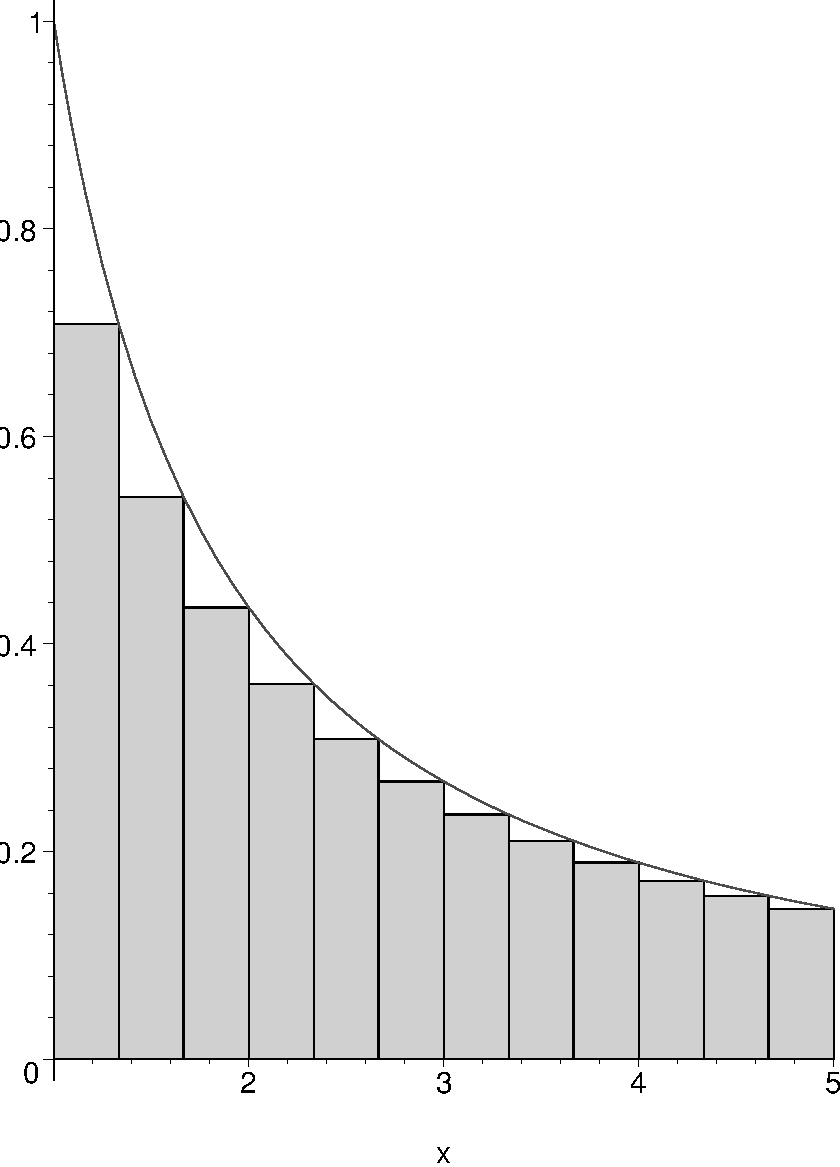
\includegraphics[width=8cm, height=6cm]{images/Box12}}
\only<4>{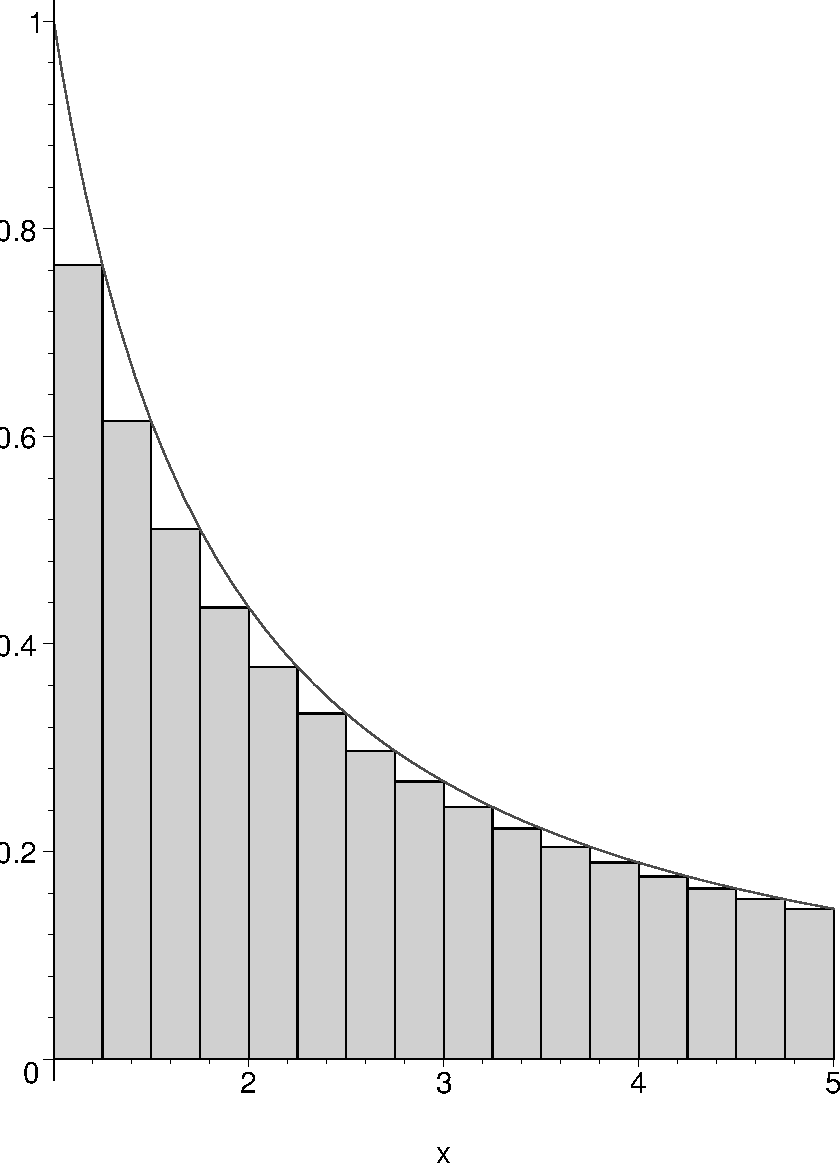
\includegraphics[width=8cm, height=6cm]{images/Box16}}
\only<6>{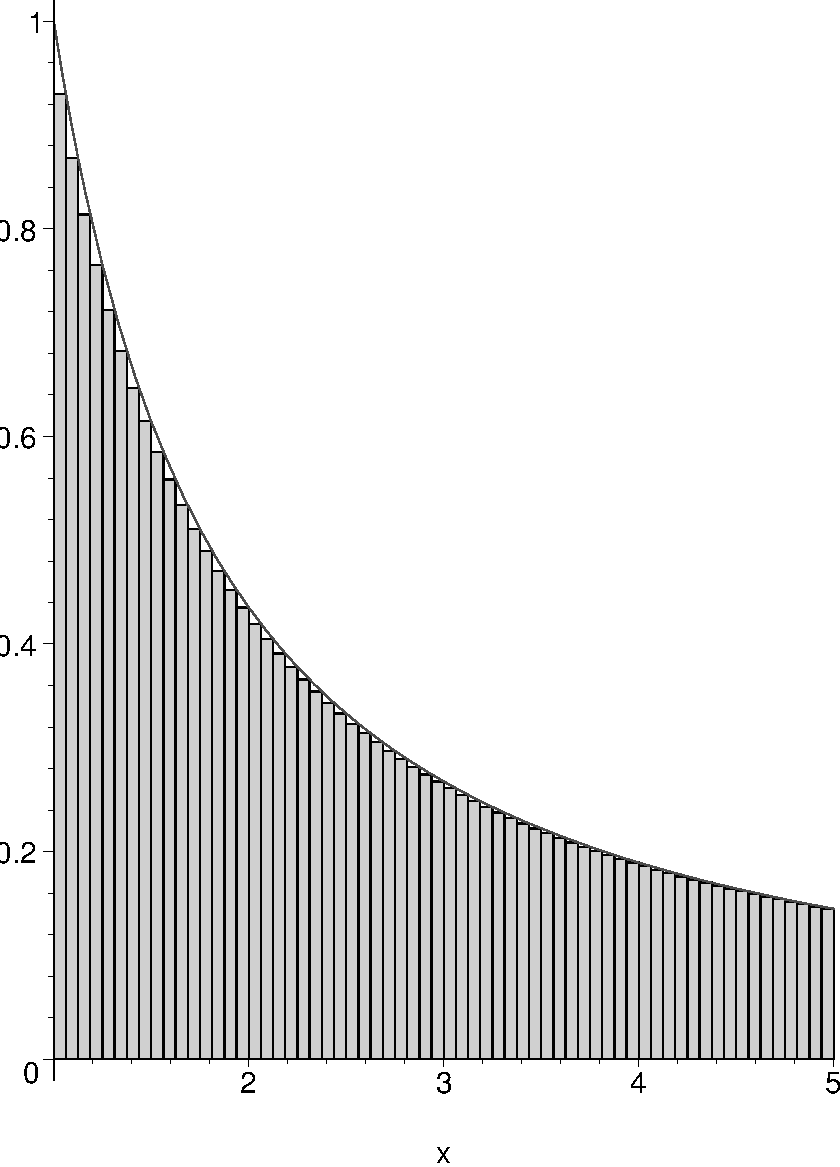
\includegraphics[width=8cm, height=6cm]{images/Box64}}
\only<7>{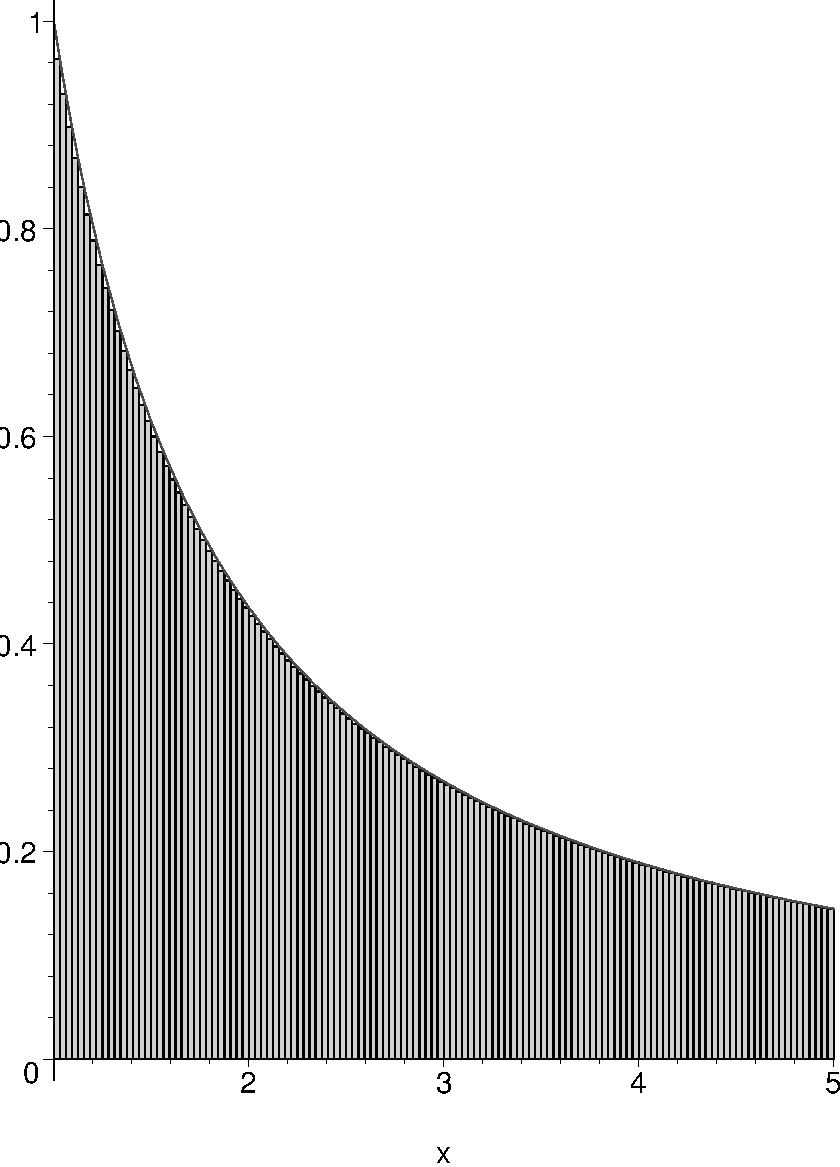
\includegraphics[width=8cm, height=6cm]{images/Box128}}
\end{center}
\vspace{-0.5cm}
\only<5>{\[Area \approx S_{32} =\sum_{k=1}^{32} A_k.\]}
\only<1>{\[Area \approx S_6 = \sum_{k=1}^6 A_k.\]}
\only<2>{\[Area \approx S_8 = \sum_{k=1}^8 A_k.\]}
\only<3>{\[Area \approx S_{12} =\sum_{k=1}^{12} A_k.\]}
\only<4>{\[Area \approx S_{16} =\sum_{k=1}^{16} A_k.\]}
\only<6>{\[Area \approx S_{64} =\sum_{k=1}^{64} A_k.\]}
\only<7>{\[Area \approx S_{128} =\sum_{k=1}^{128} A_k.\]}
}

\frame{
First we divide the interval \eq{[a,b]}:
\[
a=x_0 < x_1 < x_2 \cdots < x_n = b \quad \text{ and } \delta x = x_i
- x_{i-1} = \frac{b-a}{n}.
\]
Then the area of each box is:
\[ A_k =  f(x_k)\delta x.\]
Define the sums of the areas of \eq{n} boxes as 
\[ S_n = A_1 + A_2 + \cdots + A_n,\] 
And now:
\[
Area = \lim_{n \to \infty} S_n = \alert{\int_a^b f(x) dx}.
\]
}


\section{Definite Integrals}
\frame{
\begin{block}{}
The integral of a function \eq{f} from \eq{a} to \eq{b} 
\[
\int_a^b f(x) dx,
\]
where
\begin{itemize}
\item \eqd{\int} is the integration symbol
\item \eq{a} and \eq{b} are the lower and upper \Emph{limits of
  integration}
\item \eq{dx} means we are integrating with respect to \eq{x}.
\end{itemize}
\end{block}
}

\frame{

You should know the following properties:
\begin{itemize}[<+->]
\item \eqd{\int_{\alert{a}}^{\alert{a}} f(x) dx = 0}
\item \eqd{\int_{\alert{a}}^{\alert{b}} f(x) dx = -\int_{\alert{b}}^{\alert{a}} f(x) dx}
\item \eqd{\int_{\alert{a}}^b f(x) dx + \int_b^{\alert{c}} f(x) dx = \int_{\alert{a}}^{\alert{c}} f(x) dx}
\item \eqd{\int_a^b \alert{C} f(x) dx = \alert{C} \int_a^b f(x) dx}
  for any constant \eq{\alert{C}}.
\item \eqd{\int_a^b {\alert{f(x) + g(x)}} dx =  \int_a^b {\alert{f(x)}} dx +  \int_a^b {\alert{g(x)}} dx}
\end{itemize}
}

\frame{
\gblock
\begin{exercise}[Q16.2]
Which of the following statements is true? Why?
\[ \int_a^b |f(x)| dx \leq \bigg|\int_a^b f(x) dx\bigg|,\]
or
\[  \bigg|\int_a^b f(x) dx\bigg| \leq \int_a^b |f(x)| dx.\]
\end{exercise}
}

\subsection{The Fundamental Theorem of Calculus}
\frame{
\begin{theorem}[The Fundamental Theorem of Calculus]
Let \eq{F(x)} be defined as 
\[ F(x) = \int_a^x f(x) dx. \]
Then $F'(x) = f(x)$. That is
\[ \frac{d}{dx} \int_a^x f(x) dx = f(x). \]

Furthermore, let  \eq{g(x)} be \emph{any} antiderivative of
  \eq{f}. That is: \eq{G'(x)=f(x)}. Then
\[
\int_a^b f(x) dx = G(b) - G(a) \pause := G(x)\bigg|_a^b.
\]

\end{theorem}
}

\subsection{Examples}
\frame{

\begin{block}{}
To evaluate a definite integral of the form 
\[ \int_a^b f(x) dx,\]
find an anti-derivative \eq{G} of \eq{f} so that \eq{G'(x) =
  f(x)}. Then 
\[
\int_a^b f(x)dx = G(b) - G(a). 
\]
\end{block}
}

\frame{

\begin{example}
Evaluate each of the following
\[ 
(\alert{a}) \int_0^2 x^2 dx; \qquad 
(\alert{b}) \int_{1}^{2} \frac{(x +2)^2}{x} dx;  \qquad 
(\alert{c}) \int_0^{\pi} \sin(\frac{x}{3}) dx. 
\]
\end{example}
\vspace{4cm}
}


\subsection{The Mathematical Tables}

\frame{

In these examples we relied on knowing the anti-derivative of some
elementary  functions.

If you don't remember these, or others, look them up on pages 41 and 42 of the Mathematical Tables.


}

\frame{
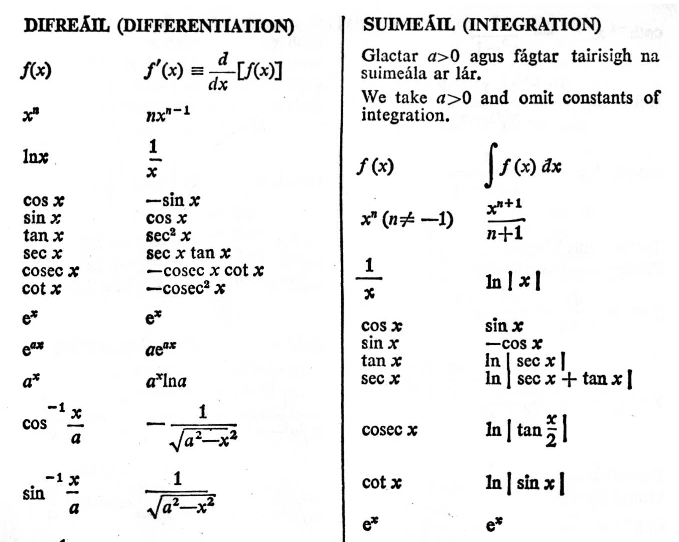
\includegraphics[width=10cm]{images/p41a}
}

\frame{
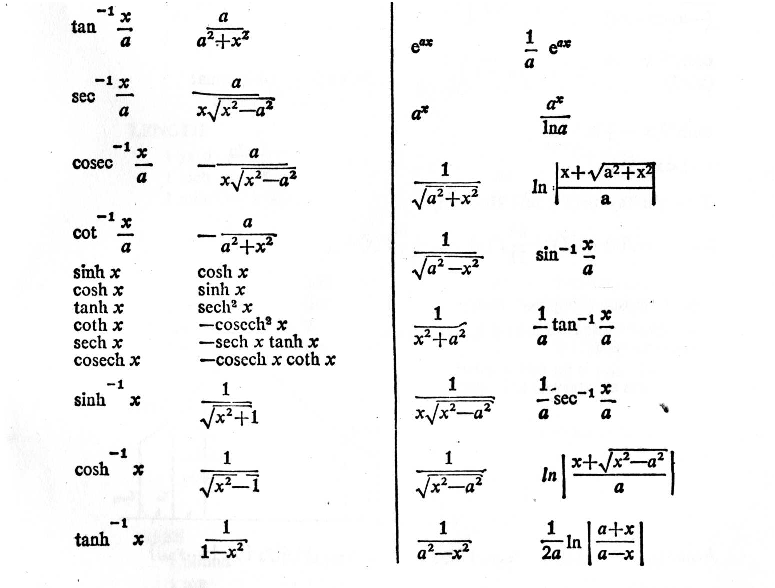
\includegraphics[width=10.5cm]{images/p41b}
}

\frame{
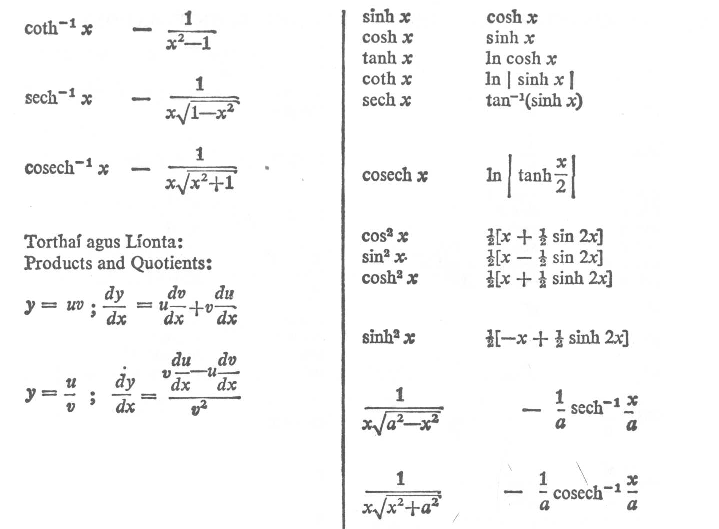
\includegraphics[width=10.5cm]{images/p42a}
}

\end{document}
\frame{

\begin{example}[Q1(c)(iv), Autumn, 05/06]
Evaluate the following integral:
\eqd{ \int \tan^2 (x) dx.}
\end{example}
\vspace{4.5cm}
}



\frame{

In most cases, we can't just look-up the answer in a table.
We may have to simplify the express, e.g., using Partial Fractions, or
(more often) using a \Bf{Substitution}.

}

\section{Method of Substitution}

\frame{

\rblock
The method of substitution comes from the \Emph{Chain Rule of
  differentiation} and is summarised as

\begin{block}{Substitution}
Let \eq{u=g(x)}. The \eq{du = g'(x) dx}. So
\[
\int f'( g(x))g'(x) dx = \int f'(u)du = f(u) + C = f(g(x)) + C.
\]\end{block}

}

\subsection{Examples}


\frame{
\begin{example}
Evaluate the indefinite integrals\\
\[ 
(i) ~~ \alert{\mathcal{I}} = \int \sqrt{x+3}  dx. \pause
\qquad 
(ii) ~~ \alert{\I}= \int \frac{1}{\sqrt{x+3}}  dx.
\]
\end{example}

\vspace{5cm}

}




\frame{
\begin{example}[Q1(c)(iv), Semester 1, 06/07]
Evaluate the following integral:
\quad \eqd{ \alert{\I} = \int  \sec^4 (x) dx.}
\end{example}
\vspace{4.5cm}
}





\frame{
\begin{example}
Evaluate the indefinite integral \quad \eqd{\alert{\I} = \int \frac{x}{x^2 +1} dx.}
\end{example}

\vspace{5cm}

}

\frame{
\begin{example}
Evaluate the indefinite integral \eqd{\int \frac{\sin(3 \ln x)}{x} dx.}
\end{example}

\vspace{5cm}

}

\frame{
\begin{exercise}[16.3]
Evaluate the following integrals:
\begin{enumerate}[(i)]

\item \eqd{\int \frac{1+x}{\sqrt{1+x}} dx}.
\hspace{1.65cm}
(ii)~ \eqd{ \int  e^{(2x-2)} dx.}

\item[(iii)] \eqd{ \int  \frac{\sin(1/x)}{x^{2}} dx.}
\hspace{1.5cm}
(iv)~ \eqd{ \int e^{\sin(x)}\cos(x) dx}

\end{enumerate}
\end{exercise}

~


\begin{exercise}[16.4]
Use a suitable substitution to show that 
\[ \int \frac{1}{\tan(x)} dx = \ln |\sin(x)|.\]
\end{exercise}
\pause
\Emph{Hint:}

}

\end{document}
